\documentclass[titleunderline,widescreen1610]{chalmerspresentation}

\usepackage{enumerate}
\usepackage{overpic}
\usepackage{siunitx}

\newcommand{\DREAM}{\textsc{Dream}}

% Unknown quantities
\newcommand{\Efield}{E_\parallel}
\newcommand{\fhot}{f_{\rm hot}}
\newcommand{\fre}{f_{\rm RE}}
\newcommand{\Ip}{I_{\rm p}}
\newcommand{\ncold}{n_{\rm cold}}
\newcommand{\nhot}{n_{\rm hot}}
\newcommand{\ions}{n_{\rm i}}
\newcommand{\nre}{n_{\rm RE}}
\newcommand{\ntot}{n_{\rm tot}}
\newcommand{\jhot}{j_{\rm hot}}
\newcommand{\johm}{j_{\Omega}}
\newcommand{\jtot}{j_{\rm tot}}
\newcommand{\psiedge}{\psi_{\rm edge}}
\newcommand{\Vloopwall}{V_{\rm loop, wall}}
\newcommand{\psip}{\psi_{\rm p}}
\newcommand{\Tcold}{T_{\rm cold}}
\newcommand{\Wcold}{W_{\rm cold}}

\newcommand{\phat}{\hat{\bb{p}}}
\newcommand{\pmax}{p_{\rm max}}
\newcommand{\Vp}{\mathcal{V}'}
\newcommand{\VpVol}{V'}

\title{The dreamers guide to runaway physics}
\coauthors{\noindent O.~Embreus and M.~Hoppe}
\frontimage{../../../media/logo1.pdf}
\titledisplacement{1mm}

% Block template

\begin{document}
    {
        \begin{frame}
            \titlepage
        \end{frame}
    }

    \begin{frame}{Features and buzzwords}
        \begin{itemize}
            \item Fully implicit, non-linear, self-consistent solver for runaway generation during tokamak disruptions \emph{(time-linearized mode also available)}
            \item Numerical conservation of particle number and positivity
            \item Flux-averaged and bounce-averaged treatment of dynamics (``1.5D'')
            \item Treating electrons as up to 4 separate populations (thermal, hot-tail, kinetic runaway, fluid runaway)
            \item Two-component code
            \begin{itemize}
                \item High-performance kernel written in C++17 (with PETSc for linear algebra)
                \item User-friendly frontend written in Python
            \end{itemize}
        \end{itemize}
    \end{frame}

    \begin{frame}{Computational regions}
        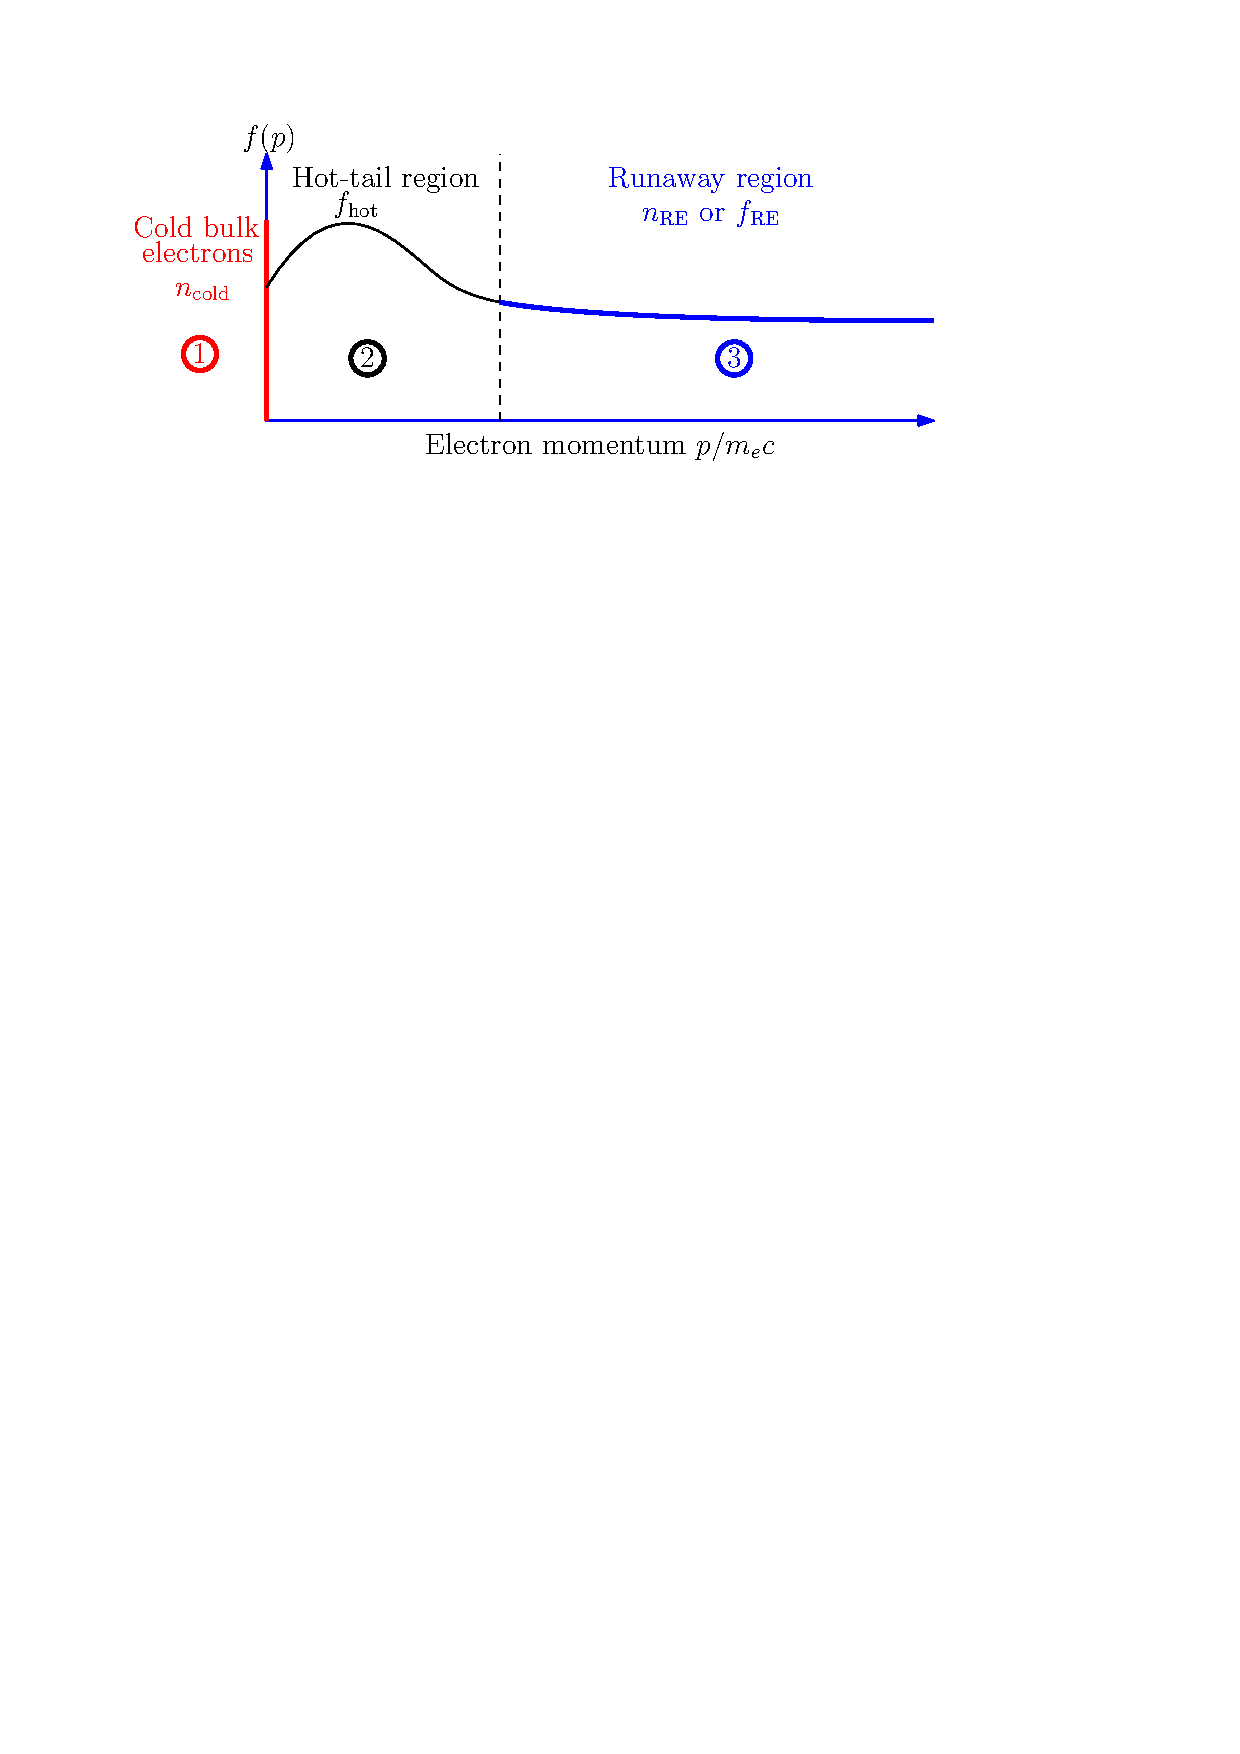
\includegraphics[width=\textwidth]{figs/regions.pdf}
    \end{frame}

    \begin{frame}{The \DREAM\ equation system}
        \begin{itemize}
            \item {\bf Scalar quantities}
            \begin{itemize}
                \item $\Ip(t)$: Total plasma current
                \item $\psiedge(t)$: Poloidal magnetic flux at plasma edge
                \item $\Vloopwall(t)$: Loop voltage at the (resistive) wall
            \end{itemize}
            %
            \item {\bf Fluid quantities}
            \begin{itemize}
                \item $\Efield(t,r)$: Parallel electric field
                \item $\ncold(t,r)$: Cold electron density
                \item $\nhot(t,r)$: Hot electron density
                \item $\ions(Z,Z_0;t,r)$: Ion (charge state) densities
                \item $\nre(t,r)$: Runaway density
                \item $\ntot(t,r)$: Total electron density
                \item $\jhot(t,r)$: Hot electron current density
                \item $\johm(t,r)$: Ohmic current density
                \item $\jtot(t,r)$: Total current density
                \item $\psip(t,r)$: Poloidal magnetic flux
                \item $\Tcold(t,r)$: Cold electron temperature
                \item $\Wcold(t,r)$: Cold electron energy content (kinetic+binding)
            \end{itemize}
            %
            \item {\bf Hot-tail grid quantities}
            \begin{itemize}
                \item $\fhot(t,r,p,\xi)$: Hot electron distribution function
            \end{itemize}
            %
            \item {\bf Runaway grid quantities}
            \begin{itemize}
                \item $\fre(t,r,p,\xi)$: Runaway electron distribution function
            \end{itemize}
        \end{itemize}
    \end{frame}

    \begin{frame}%{The \DREAM\ equation system}
        \begin{minipage}{0.48\textwidth}%
            \begin{block}{Scalars}
                \begin{itemize}
                    \item $\Ip(t)$: Total plasma current
                    \item $\psiedge(t)$: Poloidal magnetic flux at plasma edge
                \end{itemize}
            \end{block}
            \begin{block}{Densities}
                \begin{itemize}
                    \item $\ncold(t,r)$: Cold electron density
                    \item $\nhot(t,r)$: Hot electron density
                    \item $\ions(Z,Z_0;t,r)$: Ion densities
                    \item $\nre(t,r)$: Runaway density
                    \item $\ntot(t,r)$: Total electron density
                \end{itemize}
            \end{block}
            \begin{block}{Distribution functions}
                \begin{itemize}
                    \item $\fhot(t,r,p,\xi)$: Hot electrons
                    \item $\fre(t,r,p,\xi)$: Runaway electrons
                \end{itemize}
            \end{block}
        \end{minipage}%
        %
        \hfill%
        %
        \begin{minipage}{0.48\textwidth}%
            \begin{block}{Current densities}
                \begin{itemize}
                    \item $\jhot(t,r)$: Hot electron current density
                    \item $\johm(t,r)$: Ohmic current density
                    \item $\jtot(t,r)$: Total current density
                \end{itemize}
            \end{block}
            \begin{block}{Other quantities}
                \begin{itemize}
                    \item $\Efield(t,r)$: Parallel electric field
                    \item $\psip(t,r)$: Poloidal magnetic flux
                    \item $\Tcold(t,r)$: Cold electron temperature
                \end{itemize}
            \end{block}
        \end{minipage}
    \end{frame}

    \begin{frame}{Equations: (Almost) always used}
        \begin{align}
            \nhot &: \nhot = \int\fhot\,\Vp\dd p\dd\xi, \tag{$\fhot$ density moment}\\
            \nre &: \frac{\partial\nre}{\partial t} = S_{\rm ava} - \int\phat\cdot\bb{\Phi}_{\rm hot}(\pmax, \xi)\,\Vp\dd\xi, \tag{avalanche+$\fhot$ outflux}\\
            \ntot &: \ntot = n_{\rm free} + n_{\rm bound}, \tag{electron conservation}\\
            \jhot &: \jhot = \int ev_\parallel\fhot\,\Vp\dd p\dd\xi, \tag{$\fhot$ current moment}\\
            \jtot &: \jtot = \johm + \jhot + ec\nre, \tag{current conservation}\\
            %\psip &: \frac{\partial\psip}{\partial t} = V_{\rm loop}, \tag{induction}\\
            \psip &: \mu_0\frac{j_\parallel}{B}\left\langle \bb{B}\cdot\nabla\phi \right\rangle =
                \frac{1}{V'}\frac{\partial}{\partial r}\left[
                    V' \left\langle \frac{\left|\nabla r \right|^2}{R^2} \right\rangle
                    \frac{\partial\psi}{\partial r}
                \right], \tag{flux diffusion}\\
            \Ip &: \Ip = \frac{1}{2\pi}\int\jtot(r)\,\VpVol\dd r, \tag{definition of $\Ip$}
        \end{align}
    \end{frame}

\end{document}
